This chapter builds upon the insights collected in the previous chapters. Based on these findings, this study shall undertake empirical research. The concepts and techniques used to undertake the empirical research shall be discussed here. 
\section{Research design}
This study aims to investigate the long term relationship between the B-BBEE policy and firm performance. The research question and theoretical framework discussed in the previous chapter guide the operationalization which this chapter introduces to perform empirical analysis in the following chapter. This section follows this logical sequence by first revising the main research and sub research question. Thereafter the research method is presented.
\subsection{Research questions}
The main research question posed in the Introduction chapter is: “What is the long term relationship between the Broad-Based Black Economic Empowerment policy on firm performance of Johannesburg Stock Exchange-listed companies?”.  The research question indicates a generalized research. This is based analyzed through quantitative analysis seated from the theoretical framework.

To answer this research question several sub questions arise. The long term impact can be for example tested over the entire time period from 2004 to 2018. This creates the sub research question: “What was the long term relationship between Broad-Based Black Economic Empowerment policy and firm performance of the Johannesburg Stock Exchange-listed companies over the period 2004 - 2018?”.  This sub question closely resembles the research question. However, this sub research question does not answer the main research question in terms of dynamics of the long term relationship between B-BBEE policy and firm performance.

One of these dynamics, mentioned in the theoretical framework is time.  Theory concluded that B-BBEE policy intervention increased and therefore the potency of the relationship between B-BBEE policy and firm performance should increase over time. This relates to the sub research question “What was the long term relationship between B-BBEE policy and firm performance among the three B-BBEE policy periods?”. The Contextualization notes that the B-BBEE policy altered in 2004, 2007 and 2013. Thus the time period 2004 to 2018 could be subdivided into the periods 2004 - 2007, 2007 - 2013, and 2013 to 2018.

Another dynamic required to fully answer the main research question is the cross-sectional dynamics. The theory notes that the aggregate cost and benefit for firms to comply to the B-BBEE policy might differ across sectors. This relates to the sub research question: “Did the relationship between B-BBEE policy and firm performance differ across sectors?”.
\section{Research method}
This study quantitatively test the hypotheses using an ordinary least squares regression analysis. Most of the prior research on the long term relationship between B-BBEE aggregate score and share price return have deployed ordinary least squares regression analysis and no indication was presented of non-linearity of the findings. There are 2 models tested. Model 1, the FF model, resembles the Fama and French model:
\begin{equation}
\begin{aligned} %https://tex.stackexchange.com/questions/194236/why-does-not-go-to-new-line-in-equation - makes sure equation stays in marging of page
    R_{it} = R_{ft} + \beta BBBEE_{it} + \beta BBBEE_{iM}[E(R_{Mt}) - R_{ft}] \\
    + \beta_{iBP} BP_t + \beta_{iSIZE} SIZE_t +  \beta IND_{it} + \epsilon_{it}
\end{aligned}
\end{equation}
where $R_{it}$ is the share price return of observation $i$ at time $t$, $R_{ft}$ is the risk free return at time $t$, $\beta BBBEE_{it}$ is the B-BBEE rank for observation $i$ at time $t$, $\beta BBBEE_{iM}[E(R_{Mt}) - R_{ft}]$ is the (beta) coefficient of observation $i$ for the market risk premium at time $t$ over the risk free return at time $t$, $\beta_{iBP} BP_t$ is the (beta) coefficient of observation $i$  for index of high minus low book to market value at time $t$, $\beta_{iSIZE} SIZE_t$ is the (beta) coefficient of observation $i$  for the index of high minus low market capitalization at time $t$, $\beta IND_{it}$ are the coefficients of observation $i$ for the vector of industry dummy variables at time $t$ and $\epsilon_{it}$ is the error term for observation $i$ at time $t$. 

This model follows the original Fama French model by measuring the BP and SIZE factors as indices of high minus low book to market indices and high minus low market capitalization firms. It is important to note that the Fama and French model does not incorporate a constant, which is conventional in regression models. This is because the Fama and French assumes that capital markets are efficient and therefore all share price return is captured by the variables proposed \cite[]{N64}. 

Model 2, the MF model is defined similarly to the model defined by Merwe and Ferreira:
\begin{equation}
\begin{aligned} %https://tex.stackexchange.com/questions/194236/why-does-not-go-to-new-line-in-equation - makes sure equation stays in marging of page
    R_{it} = \alpha_0 + \beta BBBEE_{it} + \beta BP_{it} + \beta SIZE_{it}     + \beta EP_{it} + \beta IND_{it} + \epsilon_{it}
\end{aligned}
\end{equation}
where $R_{it}$ is the share price return of observation $i$ at time $t$, $\alpho_0$ is the constant, $\beta BBBEE_{it}$ is the B-BBEE rank  for observation $i$ at time $t$, $\beta BP_{it}$ is the (beta) coefficient of observation $i$ of book to market value of observation $i$ at time $t$, $\beta SIZE_{it}$ is the (beta) coefficient of observation $i$ to market capitalization of observation $i$ at time $t$, $\beta EP_{it}$ is the (beta) coefficient of observation $i$ to the earnings to price ratio of observation $i$ at time $t$, $\beta IND_{it}$ are the coefficients of observation $i$ for the vector of industry dummy variables at time $t$ and $\epsilon_{it}$ is the error term for observation $i$ at time $t$. This model closely follows the methodology of van der Merwe and Ferreira. 

Testing both the Fama and French model and Merwe and Ferreira model adds to the robustness of the empirical analysis. Model 1, based upon the Fama and French model could yield more observations.As only the beta coefficient to the index is required, more observations can be included. In model 2, based upon the van der Merwe and Ferreira model the book to market of a firm at a particular time is used. However, when the book to market of a firm is unavailable, then this firm at this particular time is discarded. On the other hand,  replicating the model of van der Merwe and Ferreira offers comparability. The models are used to test all the sub research questions.

Apart from the two models, a bootstrap simulation is ran to investigate the relationship between B-BBEE policy and firm performance in general and per sector. The advantage of running a bootstrap simulation is that this simulation does not require Gaussian assumptions. This adds to robustness of this study’s empirical analysis. To run the bootstrap simulation, B-BBEE observations are randomly resampled in a particular year. Then, the mean is calculated. This resampling is done 10,000 times for this particular year, resulting in a top 95\% mean and bottom 5\% of the generated means. This exercise is repeated for each of the years. These confidence intervals are not subject to normal distribution assumptions. The average performance of the top and bottom 30\% B-BBEE compliant firms for each year is then compared against the confidence intervals. A significant positive relationship is established when the top or bottom 30\% B-BBEE outperforms the top 95\%. This method resembles the bootstrap methodology used by Mehta and Ward. The selection for 30\% as the cut of for top and bottom B-BBEE was inspired by the cut off Fama and French used for the calculation of the Fama and French factors.
\subsection{Replicability}
The models, and their accompanied results were coded using Python. The repository with code is available through github at \url{https://github.com/OmegalGangapersad/MasterThesis}. This study argues that composing models in an universally popular open source coding language such as Python and making this code available for inspection by any individual through github increases the transparency and replicability of this study. 
\subsection{Defining long term}
The body of research discussed in the section “Previous research" uses a time horizon of one year to investigate the long term effect of B-BBEE on firm performance. Merwe and Ferreira (\citeyear{N7}, p554) note that using a time horizon of one year is not sufficient to capture the efficacy of the policy. This research adds to the body of research by investigating the relationship between B-BBEE rank and share price return, one, two, three, four and five years forward. The long history of B-BBEE enables this research to perform these analyses. 
\section{Variables and data collection}
This section defines the variables mentioned in the research method and provides justification for selecting these variables. Finally this section will disclose how the the data on these variables were collected. 
\subsection{Dependent variable - share price return}
This study argues that firm profitability is the best suited measurement for firm performance. Firm profitability is operationalized through share price return. Share price returns capture future profitability discounted to current market price. Further share price returns able to appreciate investment flows of institutional investors that appreciate a firm’s compliance to B-BBEE. This study, as well as most previous research, finds share price returns the most appropriate operationalisation of firm profitability.

Share price return is defined as the daily return calculated as natural log return. The returns are calculated from August to August, as proposed by Merwe and Ferreira. Considering that B-BBEE score (mentioned in the next paragraph) are released in April, the four month lag allows the market to incorporate the information of B-BBEE scores. This data is obtained through Thomson Reuters Datastream. As discussed in the section defining long term the time horizon over which this return is calculated is one, two, three, four and five years.
\subsection{Treatment variable - B-BBEE policy}
The B-BBEE policy is measured through the compliance of firms to the policy. The variable that is used to measure firm compliance to B-BBEE policy is B-BBEE aggregate score. However, rather than simply adopting this variable, this study translates set of B-BBEE aggregate scores per firm in each year to ranks, B-BBEE ranks. The aim of this study is not to identify granularity of B-BBEE aggregate score, but to understand the long term relationship between B-BBEE policy and firm performance. Using ranks rather than scores better differentiates firms in terms of compliance to the B-BBEE policy and therefore provides a better differentiating operationalization of B-BBEE compliance.

The source of the B-BBEE data from 2016 to 2018 was retrieved directly from Empowerdex through the website of their holding company, Intellidex. Colin Anthony, GM of Intellidex Investment Media, provided B-BBEE scores 2011 to 2015.  Finally, van der Merwe supplied B-BBEE scores in excel from 2005 to 2011. The source of van der Merwe was also from Empowerdex, therefore the creator of the scores was consistent, namely Empowerdex. As visualized in the below figure, the availability of BBBEE rank varied significantly by year.
\begin{figure}[!h]
  \centering
  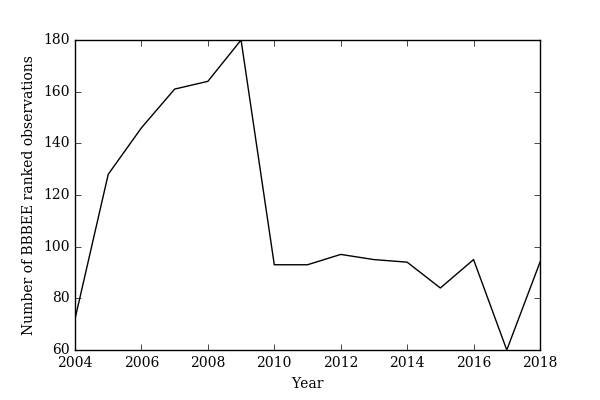
\includegraphics [scale=0.5]{ScatterPlot_Year_BBBEE_Rank.png} \\
  {\small {\it \caption{Available B-BBEE rank observations per year\label{fig:moun}}}}
\end{figure}
The B-BBEE ranks were retrieved through the Empowerdex top 100 JSE Most Empowered Companies, as mentioned in the methodology. Interestingly, it appears that the Empowerdex top 100 in pre 2010 mostly exceeded 100 firms. From 2010 onwards, the number of observations with a B-BBEE rank dropped to below 100 firms. The reason why the B-BBEE rank dropped below 100 firm, instead of equal to 100 firm as one would expect from a top 100, is that firms for which no price was available (price was retrieved from Thomson Reuters Datastream) were excluded. This resulted in an average of 5 firms being excluded, therefore an average of 95 firms available each year. Notably, in 2017 the number of firms dropped to 62. The B-BBEE rank for 2017 were retrieved from the Intellidex website. It appears that the amended codes were made obligatory by 2017, yielding in the drop of observations in 2017. The variability of observations required adjustments to prevent outcomes biased to the pre 2010 period. Put straightforward, as most observations were from pre 2010 this analysis would be moreso a reflection of the pre 2010 period, rather than the entire 2004 - 2018 period. Therefore, the number of B-BBEE rank was capped at 60, to create a uniform distribution of observations through time. In the use of the models, the B-BBEE rank was flipped, therefore rank 60 was the best ranking firm in terms of compliance to B-BBEE policy. This was done to improve readability of the regression results. In this case a negative coefficient for B-BBEE on share price returns indicates that the better the B-BBEE policy compliance of a firm, the worse the share price return.
\subsection{Control variables}
The risk free rate is defined as the yield on the 10 years South African Government bond. The yields of the 10 years South African Government bond is obtained through Thomson Reuters Datastream. The value factor is the book value per share as stated in Thomson Reuters Datastream. The book value per share equals the book market to market capitalization ratio. The size factor is the market capitalization factor and obtained through Thomson Reuters Datastream. The earnings to price ratio equals the earnings yield, which is defined as the earnings divided by the closing price of a firm. This ratio is retrieved from Thomson Reuters Datastream.

The Fama and French model uses three indices; market risk premium, BP Index and SIZE index. The constituents of these indices at any point in time depend on the universe of firms at that particular time. The availability of these firms depends on the availability of B-BBEE rank. Put straightforward, the  market risk premium is calculated as the average return of the firms available each year. The firms available each year depends on the availability of B-BBEE rank. The BP Index follows the Fama and French methodology, therefore the return of the BP Index equals the average return of the 30\% highest book to market ratio firms at a particular time minus the average return of the 30\% lowest book to market ratio firms at a particular time. The number of firms in total available, to emphasize, depends on the availability of B-BBEE rank. At the different time frames (one, two, three, four, five years) these indices represent the return of these indices over the different time frames, therefore the BP Index on a two years time frame represents the average two year return of the 30\% highest book to market ratio firms at a particular time minus the average return of the 30\% lowest book to market ratio firms at a particular time.

Instead of using industry categorization through the Code of Good Practise, this study based sector classification based on the ICB Industry name, which is gathered through the Thomson Reuters Datastream Industry Level 2 Sector Name. Using the sector classification from Thomson Reuters Datastream prevents the sector classification inconsistencies encountered in the Mokgobinyane study.
